\documentclass[11pt]{article}

\usepackage[a4paper,margin=1in]{geometry}
\usepackage[T1]{fontenc}
\usepackage[utf8]{inputenc}
\usepackage{lmodern}
\usepackage{microtype}
\usepackage{amsmath,amssymb,amsthm,mathtools}
\usepackage{booktabs}
\usepackage{array}
\usepackage{graphicx}
\usepackage{float}
\usepackage{placeins}
\usepackage{enumitem}
\usepackage[numbers,sort&compress]{natbib}
\usepackage{xcolor}
\usepackage{xurl}
\usepackage[colorlinks=true,linkcolor=blue!55!black,citecolor=blue!55!black,urlcolor=blue!55!black]{hyperref}
\usepackage[nameinlink,noabbrev]{cleveref}

\setlength{\parindent}{1.4em}
\setlength{\parskip}{0.15em}
\setlist{itemsep=0.25em,topsep=0.35em}
\allowdisplaybreaks

\newtheorem{theorem}{Theorem}[section]
\newtheorem{proposition}[theorem]{Proposition}
\newtheorem{lemma}[theorem]{Lemma}
\newtheorem{corollary}[theorem]{Corollary}
\theoremstyle{definition}
\newtheorem{definition}[theorem]{Definition}
\theoremstyle{remark}
\newtheorem{remark}[theorem]{Remark}

\newcommand{\C}{\mathbb C}
\newcommand{\Id}{\mathrm I}
\newcommand{\norm}[1]{\left\lVert#1\right\rVert}
\newcommand{\absentry}[1]{\left|#1\right|}
\newcommand{\down}{\operatorname{down}}

\hypersetup{
  pdftitle={Arcwise Primal-Dual Feshbach Enclosures at a Quadratic Band-Merging Map},
  pdfauthor={Liang Wang},
  pdfsubject={Certified rational Arnoldi relations and adaptive circular covers},
  pdfkeywords={rational Arnoldi, Feshbach map, interval enclosure, Rouché theorem}
}

\title{\textbf{Arcwise Primal--Dual Feshbach Enclosures at a Quadratic Band-Merging Map:}\\[0.35em]
\large Certified Rational Arnoldi Relations, Adaptive Circular Covers,\\
and a Single Remaining Resolvent Gate}
\author{Liang Wang\\
\small School of Artificial Intelligence and Automation,\\[-0.2em]
\small Huazhong University of Science and Technology, Wuhan 430074, P.R. China\\
\small \texttt{wangliang.f@gmail.com}}
\date{July 2026}

\begin{document}
\maketitle

\begin{abstract}
The preceding finite-dimensional calculation certified outward primal--dual
residual enclosures at contour nodes, but left two gaps before an arcwise
Rouché argument: shifted Arnoldi coordinates had only been evaluated at
nodes, and subtracting independently enclosed deep and shallow solutions
destroyed their common spectral-parameter correlation.  This paper closes
the first gap for the stored finite model.  We derive a componentwise disc
bound for $(z\Id-H)^{-1}b$ on a whole spectral disc, prove an exact
nested-Hessenberg identity for the deep-minus-base Arnoldi increment, and
cover each circular subarc by an Arb-backed complex disc.  Columnwise
relation and coupling bounds retain the small Arnoldi-tail structure.

For the exact finite model formed from the stored binary64 factors, every
accepted subarc carries an explicit bound
\[
 \norm{\widehat F_J(z)^{-1}(F(z)-\widehat F_J(z))}_2
 \leq \bar\eta_a+M\bar c_a,\qquad z\in a,
\]
where $M$ is an external upper bound for the complement resolvent
$\norm{(z\Id-B)^{-1}}_2$.  The quantity
$M_{*,a}^-=(1-\bar\eta_a)/\bar c_a$ is a downward-rounded conditional
threshold, not an estimate of that resolvent.

An adaptive dyadic cover gives a strict full-contour stored-model enclosure
at all seven archived scales $10^{-2}\geq\sigma\geq10^{-4}$, with dimensions
from 2048 to 204800.  The maximum arcwise correction ratio rises from
$4.23\times10^{-4}$ to $0.9995896$, while the minimum conditional threshold
falls from $3.97\times10^{13}$ to $1.10\times10^5$.  The finest result is a
near-boundary success and a useful map of the next obstruction, rather than
evidence of a uniform asymptotic theorem.

The result is conditional on a validated complement-resolvent upper bound
and applies only to the stored finite factors.  It does not validate the
continuous Gaussian construction, prove a contour root count, prove a
small-noise limit, or make a claim about the Riemann hypothesis.
\end{abstract}

\noindent\textbf{Keywords:} rational Arnoldi; Feshbach map; componentwise
enclosure; adaptive interval geometry; matrix Rouché theorem; nonnormal
resolvent; outward rounding.

\medskip
\noindent\textbf{MSC 2020:} 37E05; 47A10; 47A55; 47B65; 65F10; 65F15;
65G20; 65P30.

\section{Introduction}
\label{sec:introduction}

The program leading to this paper studies a packet Feshbach reduction of a
finite noisy transfer matrix near a quadratic band-merging regime.  The
ambient complement has dimension up to 204800, while the retained packet
rank is at most nine.  Earlier papers first constructed a shifted Arnoldi
Feshbach model, then enlarged a directional Rouché budget with a
primal--dual residual identity, and finally replaced ordinary binary64
residuals by outward-rounded normwise and componentwise balls
\citep{WangContourFeshbach2026,WangDirectionalRouche2026,WangPrimalDual2026,WangOutwardCode2026}.

The last paper still had a clear boundary.  It certified quantities at 32
contour nodes, not on the arcs between them.  Moreover, if $y_K(z)$ and
$y_J(z)$ were enclosed independently and then subtracted, the two discs
contained the right functions but forgot that they depend on the same
spectral parameter.  Near a projected pole this can turn a small Arnoldi
tail into an artificial $O(h)$ increment, where $h$ is the arc-disc radius.
The first prototype of the present calculation made exactly this mistake:
at $\sigma=10^{-2}$ its coarse arc bound had $\bar\eta>7$.  The nested
identity below removes that information loss.

The purpose of RH-28 is deliberately narrow:
\begin{enumerate}
 \item extend the stored rational Arnoldi relations from nodes to certified
       spectral discs;
 \item preserve the correlation of nested Arnoldi approximants;
 \item replace a uniform contour mesh by an exact adaptive circular cover;
 \item state precisely what a future complement-resolvent theorem would buy.
\end{enumerate}

The main numerical outcome is positive but not triumphant.  All seven
stored finite scales pass the strict inequality $\bar\eta<1$, yet the
finest margin is only about $4.1\times10^{-4}$.  This is a route-map result:
the arcwise extension is viable, while the remaining inverse gate and the
finite-section/continuous-model gap are still genuine.

\subsection{Scope conventions}

Here, the words exact and validated refer to the finite model whose inputs
are the stored binary64 numbers.  The sparse Gaussian matrix, computed
peripheral modes, packet synthesis and analysis matrices, and Arnoldi data
are treated as exact stored values.  The standard round-to-nearest model is
used for operation centres; radii are propagated outward with conservative
$\gamma_k$ factors and directed successor rounding
\citep{Higham2002,Rump2010,MooreKearfottCloud2009}.  We assume finite
intermediates, no overflow, and no harmful underflow.  Construction error
relative to an exact integral kernel or an analytic eigenspace is outside
the theorem.


\section{Stored rational Arnoldi Feshbach model}
\label{sec:model}

Let $B\in\C^{n\times n}$, $C\in\C^{n\times m}$,
$E\in\C^{m\times n}$, and $D\in\C^{m\times m}$ be the exact stored
finite factors.  When the complement inverse exists, the physical Feshbach
map is
\begin{equation}
 F(z)=z\Id-D-E(z\Id-B)^{-1}C.
 \label{eq:physical-feshbach}
\end{equation}
The notation is finite-dimensional; no infinite operator is implicit.

For each packet column $i$, an independent Arnoldi reduction stores a depth
$K$ basis $Q_i\in\C^{n\times K}$, a square leading Hessenberg matrix
$H_i\in\C^{K\times K}$, and an output coupling
$L_i\in\C^{m\times K}$ \citep{Saad1980}.  The stored forcing has norm
$\beta_i>0$.  The
exact algebraic relations of the stored finite model are represented by
\begin{equation}
 BQ_i=Q_iH_i+G_i,\qquad
 C_i=\beta_i q_{i,1}+d_i.
 \label{eq:stored-relations}
\end{equation}
For a depth $J<K$, write $Q_{i,J}$ and $H_{i,J}$ for leading pieces and set
\begin{equation}
 y_{i,J}(z)=(z\Id-H_{i,J})^{-1}\beta_i e_1,\qquad
 X_J(z)=\sum_i Q_{i,J}y_{i,J}(z)e_i^T.
 \label{eq:coordinates}
\end{equation}
The stored rational model is
\begin{equation}
 \widehat F_J(z)=z\Id-\widehat D
             -\sum_i L_{i,J}y_{i,J}(z)e_i^T.
 \label{eq:model-feshbach}
\end{equation}
The hat is important: $\widehat D$ and $L_{i,J}$ are stored finite-model
quantities, while $D$ and $EQ_{i,J}$ are obtained by an independent
outward factor graph.

\subsection{Primal and dual residuals}

Put $A(z)=z\Id-B$, and let $X_K(z)$ be the deep reconstruction.  Then
\begin{equation}
 r(z)=C-A(z)X_K(z)=d+G y_K(z).
 \label{eq:primal-residual}
\end{equation}
The adjoint Arnoldi model gives $Z(z)$ and
\begin{equation}
 s(z)=E^*-A(z)^*Z(z).
 \label{eq:dual-residual}
\end{equation}
The base consistency defect is
\begin{equation}
 \delta_J(z)=z\Id-D-EX_J(z)-\widehat F_J(z).
 \label{eq:base-consistency}
\end{equation}

\begin{proposition}[Primal--dual Feshbach decomposition]
\label{prop:pd-identity}
Whenever $A(z)$ is invertible,
\begin{equation}
 F(z)-\widehat F_J(z)
 =\delta_J(z)-E\bigl(X_K(z)-X_J(z)\bigr)
  -Z(z)^*r(z)-s(z)^*A(z)^{-1}r(z).
 \label{eq:pd-decomposition}
\end{equation}
\end{proposition}

\begin{proof}
From $r=C-AX_K$, $A^{-1}C=X_K+A^{-1}r$.  Also
$s=E^*-A^*Z$ gives $E=Z^*A+s^*$, hence
$EA^{-1}r=Z^*r+s^*A^{-1}r$.  Substitute these identities into
\cref{eq:physical-feshbach}, subtract \cref{eq:model-feshbach}, and use
\cref{eq:base-consistency}.
\end{proof}

\section{Correlated coordinate discs}
\label{sec:coordinates}

\subsection{A disc solve with a positive preconditioner}

Let $H\in\C^{k\times k}$, let $z_0\in\C$, and consider
$A(z)=z\Id-H$ on $|z-z_0|\leq h$.  Let $G_0$ be a floating centre
approximation to $A(z_0)^{-1}$, and define the nonnegative matrix
\begin{equation}
 N=\absentry{\Id-A(z_0)G_0}+h\absentry{G_0}.
 \label{eq:N-majorant}
\end{equation}
If $q=\norm{N}_\infty<1$, then every $A(z)G_0$ is invertible by a
positive Neumann argument.  If $\widehat y$ is the centre solve and $p$
bounds the centre residual plus the parameter term, then
\begin{equation}
 \absentry{y(z)-\widehat y}
 \leq \absentry{G_0}(\Id-N)^{-1}p.
 \label{eq:coordinate-bound}
\end{equation}
The implementation evaluates the positive inverse by an outward Neumann sum
and a geometric tail.  A parameter-dependent right-hand side is handled by
adding its componentwise radius to $p$.

\begin{lemma}[Componentwise disc solve]
\label{lem:disc-solve}
Under the hypotheses above, the right side of
\cref{eq:coordinate-bound} encloses every exact solve on the disc.  The claim
remains valid when the centre arithmetic and the right-hand side are given
by outward componentwise balls.
\end{lemma}

\begin{proof}
Write $A(z)G_0=\Id-R(z)$.  The triangle inequality gives
$\absentry{R(z)}\leq N$, so $(\Id-R(z))^{-1}$ is bounded componentwise by
$\sum_{j\geq0}N^j$.  Multiplication by $G_0$ gives
\cref{eq:coordinate-bound}.  The ball version adds the right-side radius
before the same positive solve.  Outward arithmetic only enlarges the
right-hand side.
\end{proof}

\subsection{The nested Arnoldi increment}

The leading $J\times J$ block of an upper Hessenberg matrix $H_K$ is
$H_J$.  If $\iota y_J=(y_J,0)^T$, only the first omitted subdiagonal entry
survives in $(z\Id-H_K)\iota y_J$.

\begin{proposition}[Tail-driven nested increment]
\label{prop:nested-increment}
For $y_K=(z\Id-H_K)^{-1}\beta e_1$ and
$y_J=(z\Id-H_J)^{-1}\beta e_1$,
\begin{equation}
 (z\Id-H_K)\bigl(y_K-\iota y_J\bigr)
 =h_{J+1,J}(y_J)_J e_{J+1}.
 \label{eq:nested-increment}
\end{equation}
Consequently, an enclosure for the shallow last coordinate can be used as
the right-hand side of one deep disc solve; it is not necessary to subtract
two independently widened solution discs.
\end{proposition}

\begin{proof}
The upper Hessenberg property makes all entries of row $J+1$ to the left of
column $J$ vanish except $h_{J+1,J}$, and all lower rows have zero coupling
into the first $J$ coordinates.  The first $J$ rows cancel by the shallow
equation, leaving exactly the displayed vector.
\end{proof}

\begin{remark}
The first prototype of RH-28 omitted \cref{eq:nested-increment}.  On the
$\sigma=10^{-2}$ contour it produced a worst arc ratio larger than seven.
Using the tail-driven solve reduced the same coarse-cover ratio to
$6.6\times10^{-4}$, before columnwise relation compression.  This is a
structural correction, not a change of floating precision.
\end{remark}

\section{Certified circular subarcs}
\label{sec:geometry}

Let the target contour be $\gamma(\theta)=c+Re^{i\theta}$.  For a subarc of
angular width $\Delta\theta$, the disc centred at its midpoint has geometric
radius
\begin{equation}
 \rho_{\rm chord}=2R\sin(\Delta\theta/4).
 \label{eq:chord-radius}
\end{equation}
The code evaluates the centre and this radius with Arb at 80 decimal digits,
then adds the conversion error of its stored binary64 centre.

The initial partition uses 64 equal rational turns.  A failed disc solve,
failed projected-family inverse test, or nonclosing correction ratio causes
one interval to be bisected.  If an interval is $[a/d,b/d]$ turns, its
children are
\[
 [2a/(2d),(a+b)/(2d)],\qquad
 [(a+b)/(2d),2b/(2d)].
\]
All endpoints are stored as integers.  The final coverage check is exact
rational arithmetic: sorted leaves begin at zero, meet without gaps, and end
at one full turn.

\section{Arcwise Feshbach budget}
\label{sec:budget}

For an accepted arc $a$, the coordinate discs produce a componentwise ball
for $\widehat F_J(z)$.  Let $F_a$ be its floating centre and let $\rho_a$
be a Frobenius upper bound for its radius.  An ordinary inverse of $F_a$,
together with the defect $\norm{\Id-F_aG_a}$, gives
\[
 \kappa_a\geq\sup_{z\in a}\norm{\widehat F_J(z)^{-1}}_2
\]
provided $\norm{F_a^{-1}}\rho_a<1$.  This is the small packet Neumann gate.

The relation terms are not collapsed before multiplying by coordinates.  If
$g_{ij}$ is an outward norm bound for column $j$ of $G_i$, then
\begin{equation}
 \norm{G_i y_i}_2
 \leq\sum_j g_{ij}\absentry{(y_i)_j}.
 \label{eq:column-relation}
\end{equation}
The same columnwise rule is used for $EQ_i$ and the base coupling defect.
Let $\bar r_a,\bar s_a,\bar\Delta_a$ bound, respectively, the primal
residual, dual residual, and the computable part
\[
 \delta_J-E(X_K-X_J)-Z^*r
\]
on the arc.  Define
\begin{equation}
 \bar\eta_a=\kappa_a\bar\Delta_a,\qquad
 \bar c_a=\kappa_a\bar s_a\bar r_a,\qquad
 M_{*,a}^-=\downarrow\frac{1-\bar\eta_a}{\bar c_a}.
 \label{eq:arc-budget}
\end{equation}

\begin{theorem}[Arcwise conditional Rouché gate]
\label{thm:arc-gate}
Suppose an accepted arc has finite values above, $\bar\eta_a<1$, and the
complement inverse exists on that arc with
\[
 \sup_{z\in a}\norm{A(z)^{-1}}_2<M_{*,a}^-.
\]
Then
\[
 \sup_{z\in a}
 \norm{\widehat F_J(z)^{-1}(F(z)-\widehat F_J(z))}_2<1.
\]
Consequently the matrix Rouché comparison is valid on that arc whenever the
two Feshbach maps are analytic on the relevant interior domain.
\end{theorem}

\begin{proof}
Take norms in \cref{eq:pd-decomposition}, multiply by the certified
projected inverse bound $\kappa_a$, and use
\[
 \norm{\widehat F_J^{-1}(F-\widehat F_J)}
 \leq\kappa_a\bar\Delta_a+
 \kappa_a\norm{A^{-1}}\bar s_a\bar r_a
 =\bar\eta_a+\norm{A^{-1}}\bar c_a.
\]
The strict threshold makes the right side less than one.  The final
statement is the standard matrix Rouché implication, conditional on
analyticity and the existence of the complement inverse in the interior
\citep{GohbergSigal1971}.
\end{proof}

\begin{corollary}[Full stored-contour enclosure]
If the adaptive leaves form an exact partition of the circle and every leaf
satisfies the hypotheses of \cref{thm:arc-gate}, then the conditional
Rouché inequality holds on the entire stored contour whenever
\[
 \sup_{z\in\Gamma}\norm{A(z)^{-1}}_2<\min_a M_{*,a}^-.
\]
\end{corollary}

\begin{remark}
RH-28 computes the thresholds but does not prove the displayed upper bound
for $A(z)^{-1}$.  A one-vector lower bound, a sampled inverse norm, or a
floating pseudospectral plot cannot be substituted for that missing upper
bound.
\end{remark}


\section{Numerical audit}
\label{sec:numerics}

The physical matrices, contours, and Arnoldi depths are inherited from the
seven-scale RH-24--RH-27 archive.  Each scale is rebuilt from its stored
sparse transfer matrix, its peripheral packet pair, and the same binary64
factor graph.  The primal and adjoint Arnoldi bases are retained.  Static
relation balls are formed once per scale; arc evaluations then use only
small shifted solves and small positive matrix operations.  Sixteen Linux
forked workers share the read-only large arrays by copy-on-write.

\begin{table}[H]
\centering
\caption{Full-contour stored-model arcwise audit.  Arcs means accepted
adaptive leaves, not sampled nodes.  The final two columns are conditional.}
\label{tab:scales}
\resizebox{\textwidth}{!}{%
\begin{tabular}{rrrrrrr}
\toprule
$\sigma$ & $n$ & $m$ & arcs & max level & max $\bar\eta$ & min $M_*^-$\\
\midrule
$10^{-2}$ & 2,048 & 4 & 936 & 8  & $4.2264\cdot10^{-4}$ & $3.9726\cdot10^{13}$\\
$4\cdot10^{-3}$ & 5,120 & 5 & 2,065 & 9  & $1.3301\cdot10^{-2}$ & $5.9371\cdot10^{11}$\\
$2\cdot10^{-3}$ & 10,240 & 6 & 6,368 & 11 & $4.2752\cdot10^{-2}$ & $9.9689\cdot10^{10}$\\
$10^{-3}$ & 20,480 & 7 & 8,942 & 11 & $4.0328\cdot10^{-1}$ & $3.1793\cdot10^{9}$\\
$5\cdot10^{-4}$ & 40,960 & 7 & 7,160 & 10 & $7.3662\cdot10^{-1}$ & $5.0691\cdot10^{8}$\\
$2\cdot10^{-4}$ & 102,400 & 8 & 13,440 & 11 & $9.3186\cdot10^{-1}$ & $4.0368\cdot10^{7}$\\
$10^{-4}$ & 204,800 & 9 & 29,538 & 13 & $9.9959\cdot10^{-1}$ & $1.0999\cdot10^{5}$\\
\bottomrule
\end{tabular}}
\end{table}

Every row has an exact dyadic partition check equal to one full turn.  The
maximum projected-family Neumann products are respectively
\[
 0.99960,\ 0.99990,\ 0.99983,\ 0.99987,\
 0.99992,\ 0.99930,\ 0.99889.
\]
Thus adaptive
subdivision is often driven by a conservative local inverse test, not by a
failure of the final Rouché ratio.  The maximum coordinate contractions
range from $0.9413$ at the first scale to $0.1823$ at the last; all positive
fixed-point solves terminate with an explicit geometric tail.

\begin{figure}[H]
\centering
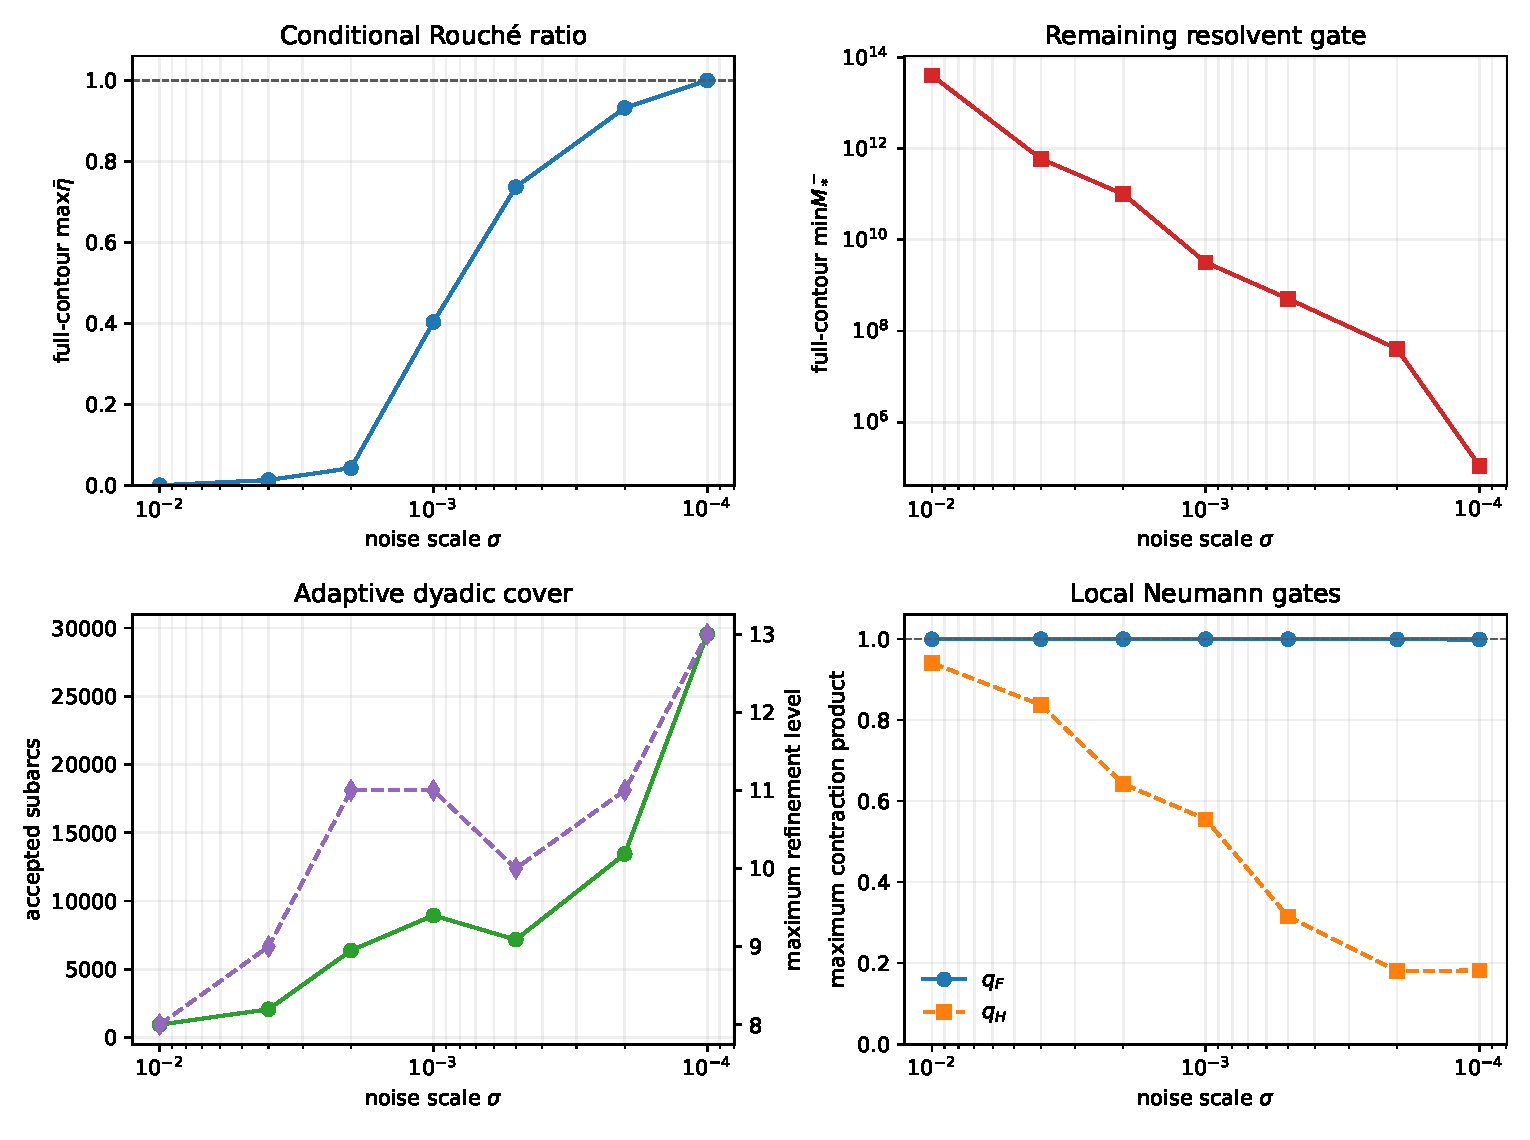
\includegraphics[width=0.98\linewidth]{figures/arcwise_scale_summary.pdf}
\caption{Arcwise correction ratios, conditional thresholds, adaptive cover
sizes, and the two local Neumann products.  The horizontal line in the top
left panel is the strict Rouché boundary $\bar\eta=1$.}
\label{fig:scale-summary}
\end{figure}

\begin{figure}[H]
\centering
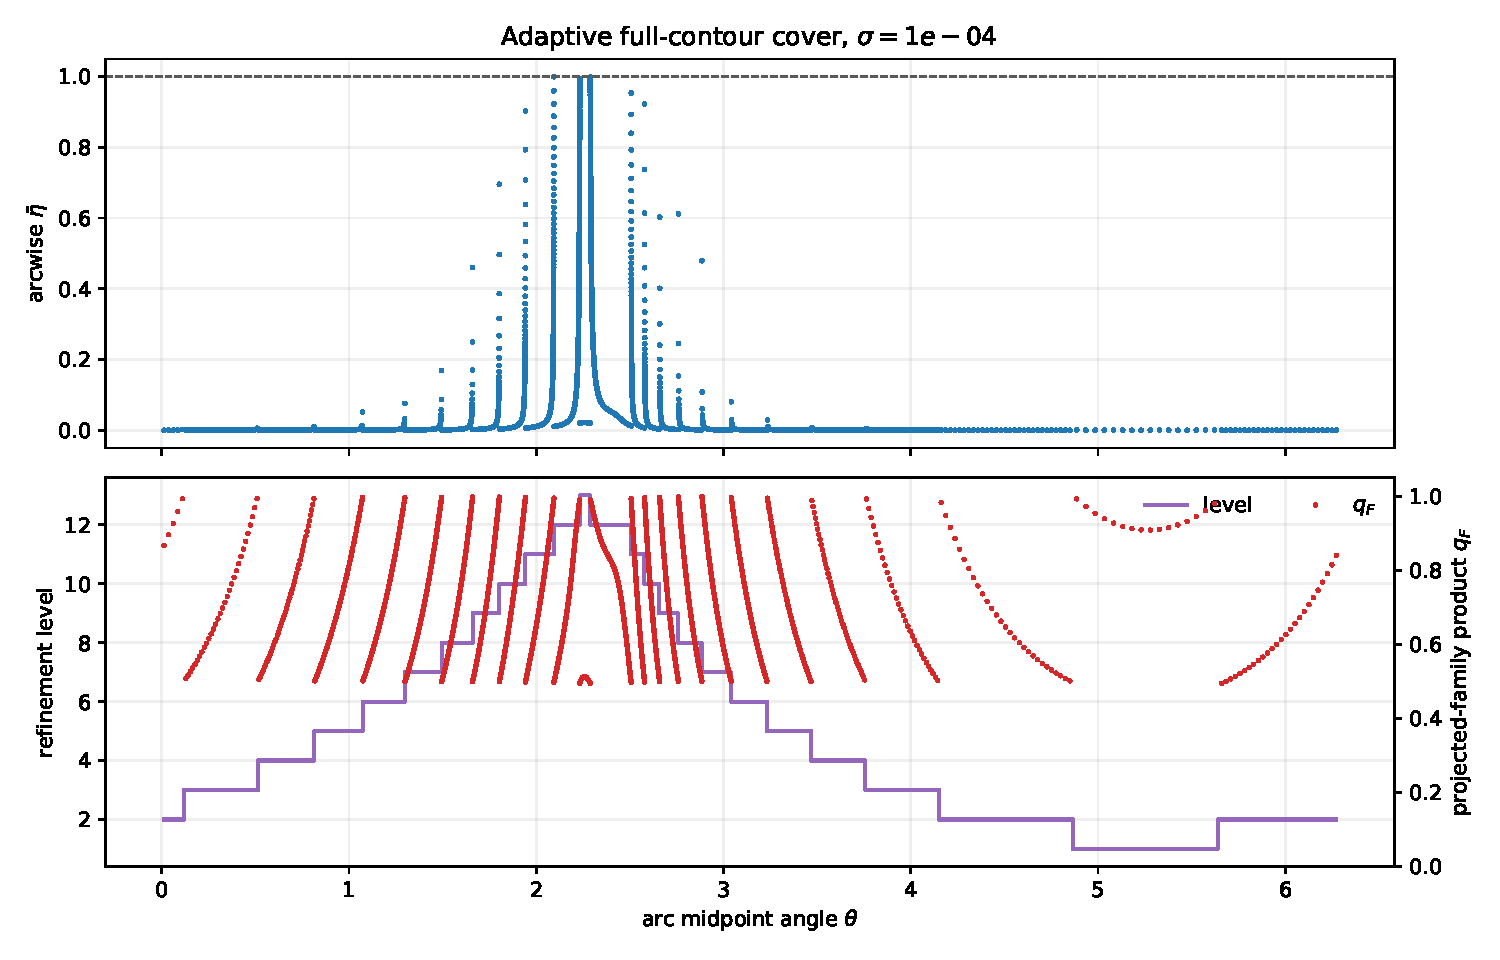
\includegraphics[width=0.98\linewidth]{figures/arcwise_finest_cover.pdf}
\caption{The finest adaptive cover.  The spikes in the upper panel identify
the difficult angular sectors; the lower panel separates the dyadic
refinement level from the projected-family Neumann product.}
\label{fig:finest-cover}
\end{figure}

The finest row is the important stress test.  The largest correction ratio
is $0.9995896159$, leaving a positive but narrow margin.  Its associated
conditional threshold is only $1.10\times10^5$, compared with
$4.04\times10^7$ one scale earlier.  This does not indicate that the
complement resolvent has reached that value; it indicates only that a future
validated upper bound must be below it to activate the conditional theorem.

\subsection{Independent checks}

The unit tests exercise the positive fixed-point solver, the nested
Hessenberg identity against sampled exact solves, Arb subarc bisection, a
small inverse family, and all seven archived exact partition certificates.
The archived tables are generated by a separate process pool from the static
relation construction, and each completed scale is written before the next
scale starts.


\section{What the result does and does not establish}
\label{sec:limits}

The result establishes a new finite-dimensional layer:
\begin{enumerate}
 \item the node-to-arc extension is no longer a mesh heuristic for the
       stored rational Arnoldi model;
 \item the nested increment is certified through an exact tail equation,
       preserving the common spectral parameter;
 \item the full circle is covered by a finite, exactly checked dyadic list;
 \item the remaining complement-resolvent requirement is reduced to an
       explicit minimum threshold at each scale.
\end{enumerate}

Several stronger statements remain unavailable:
\begin{enumerate}
 \item No upper bound for $\norm{(z\Id-B)^{-1}}$ is proved.  The archived
       $M_*^-$ values are admissible thresholds only.
 \item No winding number or root count is certified here.  A full-contour
       Rouché inequality would still need a validated base winding/root
       count and an interior analyticity argument.
 \item The finite stored factors are not enclosed relative to the exact
       Gaussian kernel, exact critical constants, or exact peripheral
       eigenspaces.
 \item No limit as $\sigma\to0$, no self-adjoint generator, no
       $T\log T$ law, and no relation to Riemann zeros is proved.
\end{enumerate}

The near-boundary finest result is therefore preferable to an optimistic
description.  It says that the arcwise route survives all seven stored
scales, but also identifies a quantitative place where the next tool must
enter.

\section{Conclusion and next gate}
\label{sec:conclusion}

RH-28 advances the program from certified contour nodes to a certified
full-contour cover for the stored rational Arnoldi model.  The key move is
not simply increasing the number of nodes.  It is preserving two kinds of
structure: the spectral-parameter correlation in the nested Arnoldi
increment, and the columnwise localization of relation and observation
defects.  Without the first, the coarsest prototype failed by orders of
magnitude; with both, all seven scales satisfy $\bar\eta<1$.

The next gate is sharply isolated:
\[
 \text{validated complement-resolvent upper bound}
 \quad <\quad \min_a M_{*,a}^-.
\]
At the finest stored scale the right side is only $1.10\times10^5$, so a
crude global estimate will not suffice.  Possible routes include a validated
block-Grushin inverse, a complement Schur resolvent estimate, or a
componentwise interval Krylov enclosure.  Any such result would still have
to be combined with a validated base winding/root count and an interior
finite-section argument.  Those are subsequent problems, not consequences
of the present paper
\citep{SjoestrandZworski2007,TrefethenEmbree2005}.

\appendix

\section{Outward arithmetic conventions}
\label{app:arithmetic}

For nonnegative stored bounds, every scalar addition and multiplication is
followed by a successor operation toward $+\infty$.  A real or complex dot
product of length $k$ is inflated by a conservative $\gamma_k$ factor;
complex magnitudes and Frobenius reductions receive separate reduction
guards.  The positive fixed-point solver computes
\[
 p+Np+\cdots+N^\ell p
\]
and adds $q\max(N^\ell p)/(1-q)$ componentwise as a geometric tail.  A failed
contraction is not converted into a numerical value: it triggers arc
bisection.

The small inverse certificate uses an ordinary centre inverse only as a
preconditioner.  If $X$ is that inverse and
$d=\norm{\Id-F_aX}$ is outwardly bounded by $d<1$, then
\[
 \norm{F_a^{-1}}_2\leq\frac{\norm{X}_2}{1-d}.
\]
For a componentwise family radius $\rho_a$, the same argument gives the
family bound used in \cref{sec:budget} when
$\norm{F_a^{-1}}\rho_a<1$.

\section{Reproducibility}
\label{app:reproducibility}

The repository subdirectory contains the source modules, tests, archived CSV
tables, metadata, figures, and this manuscript \citep{WangArcwiseCode2026}.
From the directory, run:
\begin{verbatim}
/root/math/.venv/bin/python -m pytest -q
/root/math/.venv/bin/python experiments/make_figures.py
\end{verbatim}
The expensive audit is resumable:
\begin{verbatim}
/root/math/.venv/bin/python \
  experiments/run_arcwise_enclosure.py \
  --sigmas 0.0001 --arcs 64 --workers 16 --resume
\end{verbatim}
The process-pool implementation targets the Ubuntu/Linux environment used
for the large scales; setting \texttt{--workers 1} removes parallelism.

\bibliographystyle{unsrtnat}
\bibliography{references}

\end{document}
